\subsubsection{Generic distributed system frameworks}
Distributed system have already been implemented in the industry to solve the problem of companies possessing massive amounts of data that they want to be able to query and analyze. These frameworks largely rely on the fact that it is cheaper
to have multiple servers, each of them with a relatively small storage capacity and computing power, rather than having one expensive large server.

\paragraph{The frameworks}
The basis of existing frameworks is based on the Google File System\cite{Ghem03}. This \textit{Google File System} or \textit{GFS} is the system that is used within Google to handle all the Big data needs within the company. GFS splits all the data that is uploaded to the cluster up into chunks, which are then split over the "chunk servers" in the node. These chunks are then replicated a predefined number of times (usually 3) in order to guarantee that the data is not lost when a server fails. The data on the chunk servers can then be accessed by a user by contacting the master, which knows exactly on which servers each chunk is saved.\cite{Ghem03} The data and work-flow is described in Figure \ref{GFS_Architecture} below.

\begin{figure}
	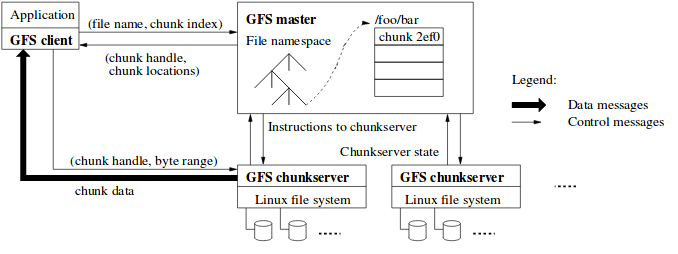
\includegraphics[width=\textwidth]{GFS_Architecture.png}
	\caption{Google File System architecture\cite{Ghem03}}
	\label{GFS_Architecture}
\end{figure}

The GFS architecture that was described in its paper by Google was adapted into an open-source solution called Hadoop \cite{Shv10}. Hadoop was developed mainly by Yahoo!, distributed as an Apache project and functions essentially the same as GFS. There are only minor differences with GFS such as the naming of certain entities and the chunk size. A typical use case of adding a file to the Hadoop File System (HDFS) is show in Figure \ref{Hadoop_usecase} below.

\begin{figure}
	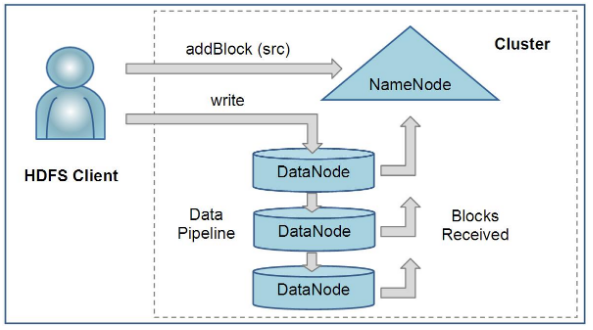
\includegraphics[width=\textwidth]{Hadoop_use_case.png}
	\caption{The data flow when adding a file to the HDFS\cite{Shv10}}
	\label{Hadoop_usecase}
\end{figure}

\paragraph{Uses of the frameworks}
The storage framework highlighted above, is the most-common file-system that empower Big Data implementations today. These implementations are frameworks such as MapReduce and the Apache Spark engine.

\paragraph{MapReduce}
MapReduce is a new framework for processing data and was developed by Google\cite{Dean04} in order to process data in a distributed setting. Firstly, in the \textit{map phase} all data is split into tuples (called key-value pairs). Then, during the shuffle phase, these key-value pairs are shuffled and passed to the \textit{reduce phase} in which a calculation (often an aggregation) is performed on them to generate the a single output value. The main benefit of this framework is that the data can be distributed across a large amount of machines (which are using for example GFS or HDFS). Additionally, instead of communicating the data between the nodes, the program is communicated between the nodes which is magnitudes smaller and more efficient to pass around. A general overview of the execution of a map-reduce problem is given in Figure \ref{mapreduce_execution}.

\begin{figure}
	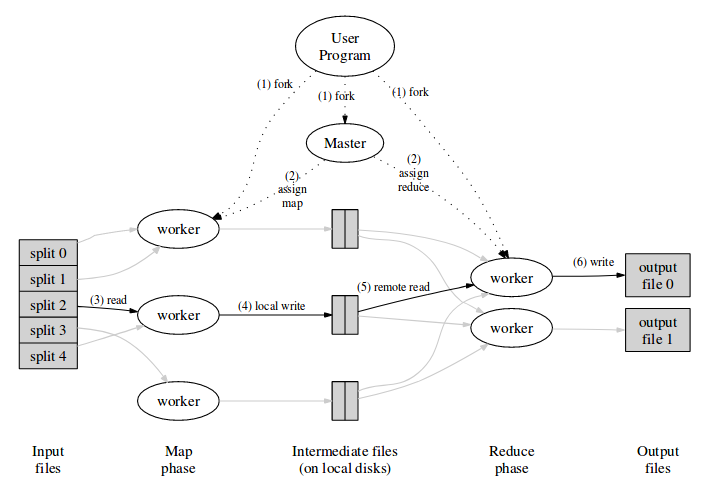
\includegraphics[width=\textwidth]{mapreduce_execution.png}
	\caption{Overview of the execution of a mapreduce problem\cite{Dean04}}
	\label{mapreduce_execution}
\end{figure}

Furthermore the MapReduce framework is similar to the \textit{Bulk-Synchronous processing (BSP)} style which is a little older. However, there are some differences as the MapReduce framework does not allow communication between nodes in the map phase, but only allows communication during the shuffle phase, in-between the mapping and reduce phase\cite{Pace12}.\\
Since BSP and Map-reduce are so similar, people have worked on transforming BSP tasks into MapReduce tasks. Goodrich et al.\cite{Goo11} has shown that all BSP programs can be converted into MapReduce programs and other researchers have even gone as far as to say that all MapReduce task are so similar to BSP tasks that, because BSP has a more theoretical basis, all tasks should be modeled as BSP tasks but implemented using the Map-reduce framework in order to gain the speed of MapReduce and the correctness of BSP\cite{Pace12}.

\paragraph{Apache Spark}
Like MapReduce, Apache Spark is another service built on top of a distributed file system to run programs on a distributed dataset. Spark is an open-source cluster-computing framework that is capable of executing an entire directed acyclic graph of transformations (like mappings) and actions (like reductions) fully in memory\cite{Sparkwebsite}. This is contrast to MapReduce, that forces the programmer to first use a mapping phase and then a reduce phase. This way, Spark is a lot faster than MapReduce because when, for example, 2 mapping phases are needed, 2 MapReduce tasks need to be executed which both require to write all (intermediate) data to the disk. Spark on the other hand can keep all the data in-memory which saves expensive writes to the disk, but needs to take additional steps to prevent losing processed data when there's a power outage.\\

The way in which Spark solves this problem is by using \textbf{RDDs} (Resilient Distributed Datasets). These datasets are read-only and new ones can only be created from data stored on the disk, or transforming existing RDDs\cite{Zaha12}. The Resilient part comes into play when the data is lost. This is done by giving each RDD a lineage graph that shows what transformations have been executed on it. This lineage graph ensures that if some data is lost, Spark can trace the path that RDD has followed by using the lineage graph and recalculate any lost data. It is important that the lineage graph does not conty cycles, i.e. is a Directed Acylic Graph (DAG), because otherwise the data cannot be recovered since Spark will run into an infinite loop.

\begin{figure}
	\begin{center}
		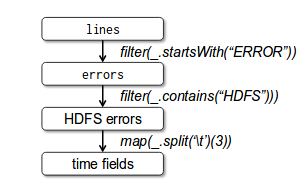
\includegraphics[scale=0.5]{Lineage_graph.png}
	\end{center}
	\caption{Example of the lineage graph of an RDD\cite{Zaha12}}
	\label{lineagegraph}
\end{figure}
